%% ****** Start of file aiptemplate.tex ****** %
%%
%%   This file is part of the files in the distribution of AIP substyles for REVTeX4.
%%   Version 4.1 of 9 October 2009.
%%
%
% This is a template for producing documents for use with 
% the REVTEX 4.1 document class and the AIP substyles.
% 
% Copy this file to another name and then work on that file.
% That way, you always have this original template file to use.

%\documentclass[aip,graphicx]{revtex4-1}
%\documentclass[aip,reprint]{revtex4-1}

%\usepackage{graphicx}

%\draft % marks overfull lines with a black rule on the right
%\documentclass[pre,aps,floatfix,authordate1-4,twocolumn]{revtex4-1}
%\documentclass[pre,aps,floatfix,authordate1-4]{revtex4-1}

\documentclass[aps,prl,superscriptaddress,twocolumn]{revtex4}



%\documentclass[aps,prl,preprint,groupedaddress]{revtex4}

\usepackage{rotating} 
\usepackage{times}
\usepackage{graphicx}
\usepackage{setspace}
\usepackage{amsmath}
\usepackage{epstopdf}
\usepackage[obeyFinal]{easy-todo}
\begin{document}

% Use the \preprint command to place your local institutional report number 
% on the title page in preprint mode.
% Multiple \preprint commands are allowed.
%\preprint{}

\title{NMRlipids IV: Other than PC headgroups} %Title of paper

% repeat the \author .. \affiliation  etc. as needed
% \email, \thanks, \homepage, \altaffiliation all apply to the current author.
% Explanatory text should go in the []'s, 
% actual e-mail address or url should go in the {}'s for \email and \homepage.
% Please use the appropriate macro for the type of information

% \affiliation command applies to all authors since the last \affiliation command. 
% The \affiliation command should follow the other information.

\author{O. H. Samuli Ollila}
\email[]{samuli.ollila@helsinki.fi}
%\homepage[]{Your web page}
%\thanks{}
%\altaffiliation{}
\affiliation{University of Helsinki}


% Collaboration name, if desired (requires use of superscriptaddress option in \documentclass). 
% \noaffiliation is required (may also be used with the \author command).
%\collaboration{}
%\noaffiliation

\date{\today}

\begin{abstract}
% insert abstract here
  Primarily measured but also simulated NMR order parameters will be collected also for other than phophatidylcholine
  (these are discussed in NMRlipids I) headgroup. The information will be used to understand structural differences between 
  different lipid molecules in bilayers.
\end{abstract}

%\pacs{}% insert suggested PACS numbers in braces on next line

\maketitle %\maketitle must follow title, authors, abstract and \pacs

% Body of paper goes here. Use proper sectioning commands. 
% References should be done using the \cite, \ref, and \label commands


%\label{}
\section{Introduction}
Phospholipids containing various polar headgroups and acyl
chains are essential building blocks of biological membranes.
Atomistic level structural details of lipids and lipid-ion 
interactions are considered highly important in several
biological processes. The lipid structure and ion binding
can be studied in detail with NMR spectroscopy. However,
the structural interpretation of NMR data requires usage
of models. The combination of classical molecular dynamics
simulations with NMR data, especially with C-H bond
order parameters, can potentially give atomistic resolution
interpretation of structure and dynamics of molecules \cite{botan15,ollila16,ferreira16}. 

Our recent studies concluded that MD models are cabable to
give structural interpretation for phosphatidylcholine 
hydrophopic acyl chain region, while hydrophilic headgrop, glycerol 
backbone and cation binding posed a major challenge for current
force fields \cite{botan15,ollila16,catte16,ferreira16}. 
These conclusions were reached by reviewing extensively 
available experimental data from various sources and using
NMRlipids Open Collaboration project to collect massive 
amount of simulation data \cite{botan15,catte16}.

Here we apply the same approach in search of MD simulation
models which would reproduce glycerol backbone and 
headgroup structures of lipids with PE, PG and PS headgroups.  
In addition, we attempt to find a MD simulation model
that would be able to correctly describe cation binding in
bilayer containing negatively charged PG and PS lipids.


%Several MD simulation models have succesfully described 
%acyl chain structures and their qaulitative changes in different
%conditions for phosphatidylcholine lipids (for review see \cite{ollila16}).
%However, the current simulation models were not found to be accurate
%enough for full structural interpretation of phosphatidylcholine headgroup and
%glycerol backbone \cite{botan15}. Also Na$ +$  binding affinities
%were found to be significantly overestimated in several models and 
%none of the available models was able to Ca$2+$ 

%\section{Methods}

%\subsection{Molecular dynamics simulations}

\section{Experimental glycerol backbone and headgroup order parameters for PE, PG and PS lipids}

Experimental order parameters for different lipid headgroups are
collected in Fig. \ref{HGorderParameters}.
\begin{figure}[]
  \centering
  \includegraphics[width=9.0cm]{../Figs/HGorderparameters.eps}
  \caption{\label{HGorderParameters}
    Order parameters for headgroup and glycerol backbone with different headgroups
  }
\end{figure}

\section{Glycerol backbone and headgroup order parameters for PE, PG and PS lipids in simulations}

\todo{Simulation data for lipids with different headgroups to be collected}

\section{Ca$2+$ binding in bilayers with negatively charged PG and PS lipids}

Ion binding affinity in lipid bilayer containing PC lipids can be 
measured by using C-H bond order parameters for headgroup $\alpha$ and
$\beta$ carbons by using the electrometer concept. The decrease of these 
order parameters is linearly proportional to the amount of bound charge 
in bilayer \cite{??,catte16}. The electrometer concept can be used also
for bilayers containing PC lipids mixed with charged lipids \cite{macdonal87,roux90,??}.
This is demonstrated in Figs \ref{OrderParametersWithCaCl},
\ref{OrderParametersWithCaClBELOW1M} and \ref{OrderParameterCHANGESWithCaClBELOW1M}, where PC headgroup order parameters 
as a function of CaCl$_2$ concentration are shown from experiments with POPC and PS or PG.
\begin{figure}[]
  \centering
  \includegraphics[width=9.0cm]{../Figs/LIPIDSwithCaCl.eps}
  \caption{\label{OrderParametersWithCaCl}
    PC headgroup order parameters as a function of CaCl concentration from experiments containing charged lipids.
    Pure DPPC data from \cite{akutsu81}, pure POPC data from \cite{altenbach84}, 
    POPC:POPS mixture data from \cite{roux90} and POPC:POPG mixture data from \cite{macdonald87}.
  }
  \todo{Check the NaCl concentrations in the samples.}
\end{figure}
\begin{figure}[]
  \centering
  \includegraphics[width=9.0cm]{../Figs/LIPIDSwithCaClBELOW1M.eps}
  \caption{\label{OrderParametersWithCaClBELOW1M}
    Figure \ref{OrderParametersWithCaCl} zoomed to smaller concentrations.
  }
\end{figure}
\begin{figure}[]
  \centering
  \includegraphics[width=9.0cm]{../Figs/CHANGESwithCaClBELOW1M.eps}
  \caption{\label{OrderParameterCHANGESWithCaClBELOW1M}
    Changes in order parameters
  }
\end{figure}

Order parameters increase when PS or PG are mixed with PC 
in the absence of additional ions, as seen from Figs. 
\ref{OrderParametersWithCaCl} and \ref{OrderParametersWithCaClBELOW1M}.
In electrometer concept this is explained by the tilting of
headgroup more parallel to membrane normal \cite{??}.
The order parameter decrease with increasing CaCl$_2$ concentration 
is explained by the tilting of headgroup more perpendicular
to membrane normal. This decrease is shown to be a good measure
for the amount of bound ions in lipid bilayer with PC lipids \cite{??,catte16}.

The order parameter decrease as a function of added CaCl$_2$
for systems with different amount of negative charge are shown 
in Fig. \ref{OrderParameterCHANGESWithCaClBELOW1M}.
As expected, the order parameter decrease is more 
pronounced with increasing amount of negatively charged lipids in
bilayer. This is explained by the increase of cation concentration
in proximity of bilayer containing negatively charged lipids \cite{??}.

In addition to the changes in PC headgroup order parameters with 
ion binding, also changes in PS and PG headgroup order parameters
are measured.
\todo{Add this data}.

\section{Ca$2+$ binding in bilayers with negatively charged PG and PS lipids in simulations}

\todo{Simulation data for systems with negatively charged lipids and CaCl$_2$ to be collected}

\section{Conclusions}

% Tables may be be put in the text as floats.
% Here is an example of the general form of a table:
% Fill in the caption in the braces of the \caption{} command. Put the label
% that you will use with \ref{} command in the braces of the \label{} command.
% Insert the column specifiers (l, r, c, d, etc.) in the empty braces of the
% \begin{tabular}{} command.
%
% \begin{table}
% \caption{\label{} }
% \begin{tabular}{}
% \end{tabular}
% \end{table}

% If you have acknowledgments, this puts in the proper section head.
\begin{acknowledgments}
% Put your acknowledgments here.
\end{acknowledgments}
\newpage
\appendix
\begin{center}
{\bf SUPPLEMENTARY INFORMATION}
\end{center}


% Create the reference section using BibTe
\bibliography{refs.bib}

%\newpage
%\section{APPENDIX: The NMR results reported by Tiago Ferreira}

\listoftodos

\end{document}
%
% ****** End of file aiptemplate.tex ******
